\chapter{2048を解くためのアプローチ}
\label{chap:rl}
これまでに2048を対象とした強化学習の研究は数多くなされてきた. 
本章では強化学習の概要, および2048に対する強化学習の先行研究について記述する.

\section{強化学習の概要}
\label{sec:rl_general}
まず本節では2048との関係を踏まえつつ, 一般的な強化学習の概要について記述する.
なお本節の内容は全体に文献~\cite{Sutton1998}および文献~\cite{deepRL}を参照して書かれた.

\subsection{マルコフ決定過程}
\label{subsec:mdp}
強化学習は与えられた環境において試行錯誤することを通して, 目標を達成するための戦略や意思決定を学習するための手法である.
学習や意思決定を行う主体はエージェントと呼ばれる.
エージェントは離散タイムステップに従って行動を選択し続け, 環境とやり取りを行う.

このような問題設定はマルコフ決定過程~(MDP)~というモデルによって定式化されている.
MDPは以下の$4$つの要素で構成される. 
\begin{itemize}
  \item 状態集合\textit{S}
  \item 行動集合\textit{A}
  \item 状態遷移関数$p:S \times A \times S \rightarrow [0,1]$
  \item 報酬関数$r:S \times A \times S \rightarrow \mathbb{R}$
\end{itemize}
エージェントはステップ$t$で状態$s_t \in S$から行動$a_t \in A$を選択する.
そして確率$p(s_{t+1}|s_t,a_t)$で次の状態$s_{t+1}$に遷移し, $r(s_t,a_t,s_{t+1})$の実現値$R_{t+1}$を即時報酬として獲得する.
状態遷移関数と報酬関数は環境のダイナミクスと呼ばれることがある. 
図\ref{fig:mdp}にMDPの模式図を示す.
\begin{figure}[h]
  \centering
  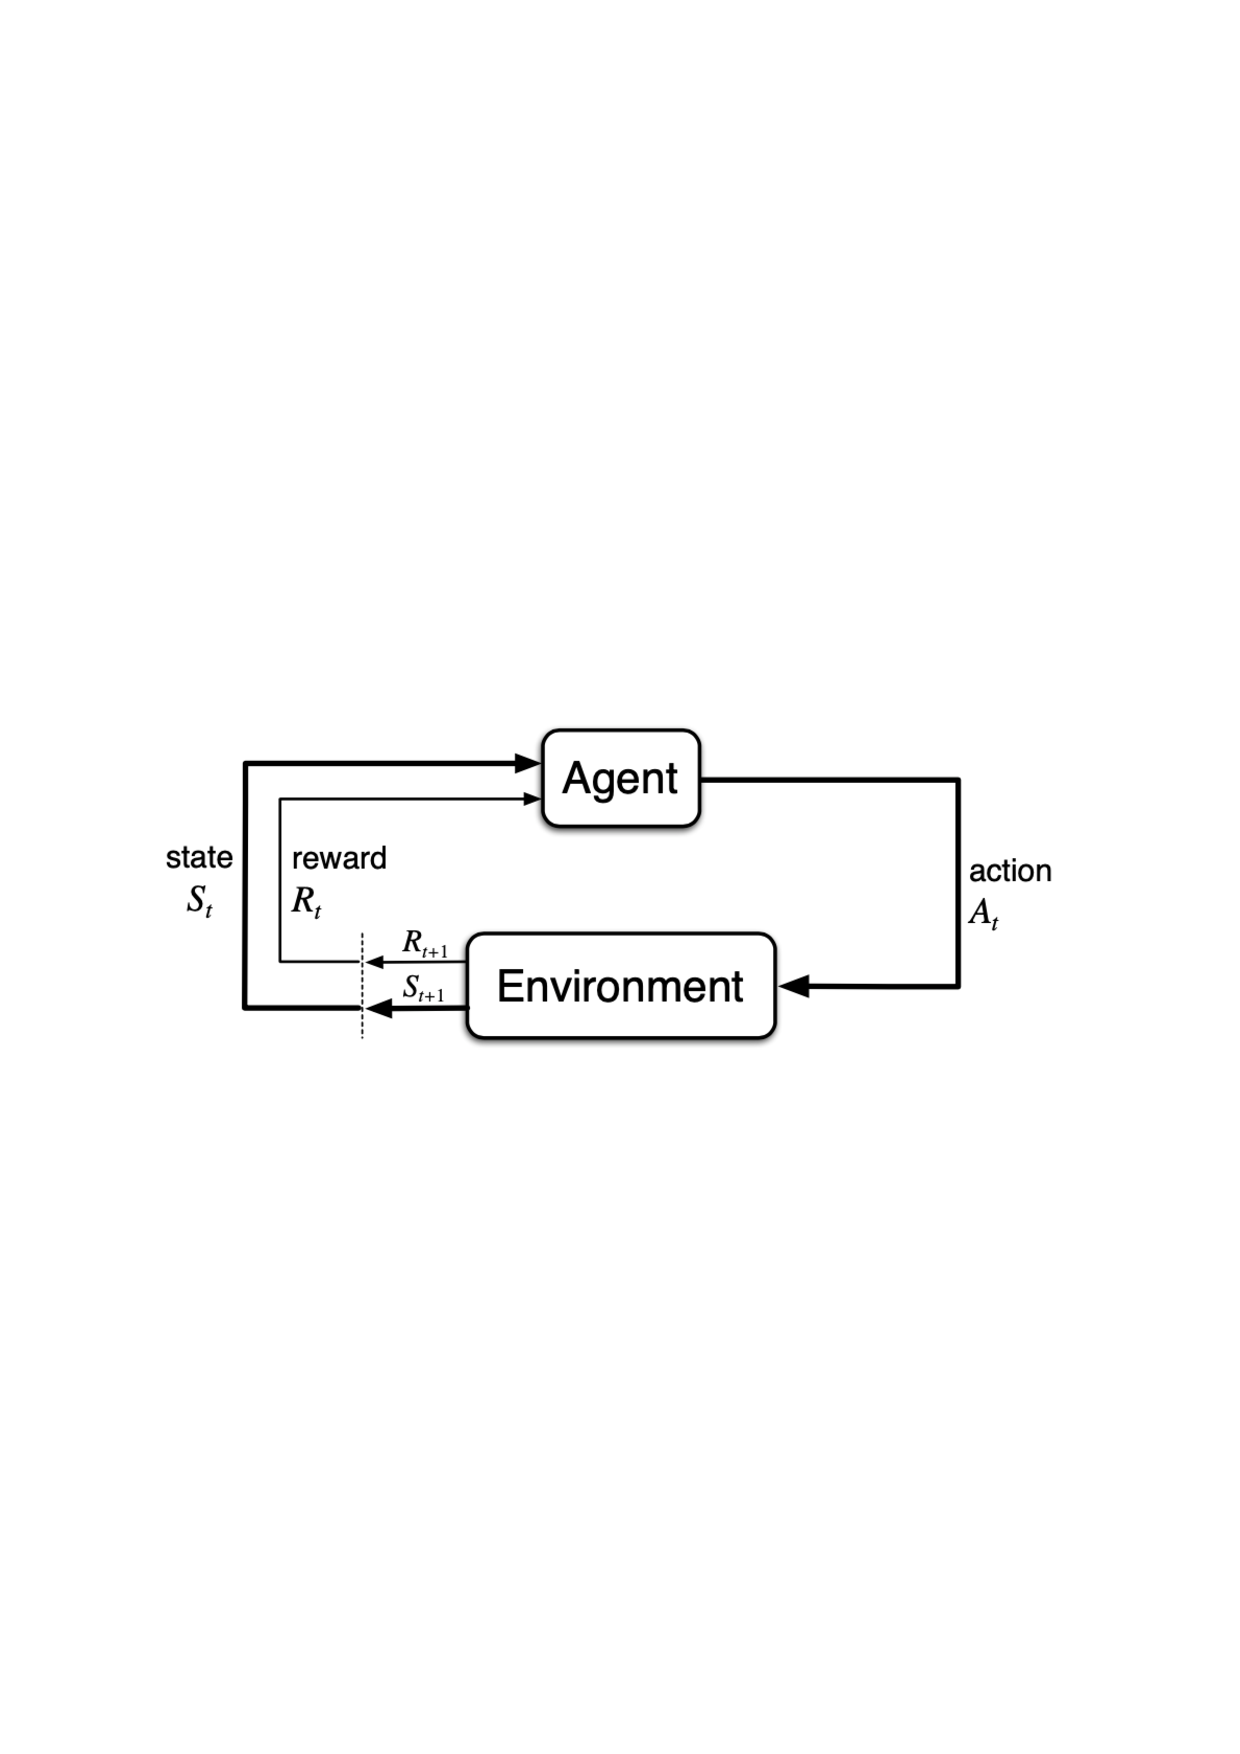
\includegraphics[width=\linewidth{}]{figures/MDP.pdf}
  \caption{MDPの模式図 (文献\cite{Sutton1998}より引用) \label{fig:mdp}}
\end{figure}

状態集合と行動集合が有限であるMDPを有限MDPと呼ぶ.
2048は有限MDPにそのまま当てはまるゲームである.
行動集合\textit{A}はプレイが選ぶ上下左右に対応し, 報酬はプレイヤが獲得する得点に対応する.
ここで2048では状態遷移得点の獲得の仕方は決定的であるため, 以降報酬関数$r$は決定的な関数であるものとして記述する.

一般に強化学習で扱う問題には, エージェントと環境のやり取りが終わる終了状態が存在するepisodic taskと終了状態が存在しないcontinuing taskが存在する. 
episodic taskではエージェントと環境のやり取りを初期状態から終了状態までのエピソードと呼ばれる単位で分割することができる.
\ref{sec:property}節で説明したように2048は必ず終了するゲームであるため, 以降episodic taskでの定義を確認する. 

\subsection{方策と価値関数}
エージェントがある状態において行動を決定する際の戦略, すなわち確率分布$\pi:S \times A \rightarrow [0,1]$を方策と呼ぶ.
状態価値関数$v_{\pi}(s)$は状態$s$から方策$\pi$に従って行動を選択し続けた場合の累積報酬和の期待値であり, 次のように定義される.
\begin{align}
  v_{\pi}(s) \stackrel{\mathrm{def}}{=} \mathbb{E}_{\pi}\left[\sum_{k=0}^T \gamma^k R_{t+k+1}|S_t=s \right]
\end{align}
同様に状態$s$から行動$a$を選択し, その後方策$\pi$に従って行動を選択し続けた場合の累積報酬和の期待値である行動価値関数$q_{\pi}(s,a)$の定義は以下のようになる.
\begin{align}
  q_{\pi}(s,a) \stackrel{\mathrm{def}}{=} \mathbb{E}_{\pi}\left[\sum_{k=0}^T \gamma^k R_{t+k+1}|S_t=s, A_t=a \right]
\end{align}

強化学習の目標は多くの報酬を獲得できるような良い方策を見つけることである.
価値関数の定義より2つの方策$\pi$と$\pi'$があるとすると, すべての状態$s \in S$について$v_\pi(s) \geq v_{\pi'}(s)$が成り立つならば$\pi$は$\pi'$と等価か$\pi'$よりも良い方策だと言える.
ここで他のすべての方策と比べて等価であるか, それよりも良い方策が少なくとも$1$つ存在する.
これは最適方策$\pi_*$と呼ばれる方策である.
$\pi_*$に従うときの状態価値関数は最適状態価値関数と呼ばれ, $v_{\pi_*}$で表される.
同様に$\pi_*$に従うときの行動価値関数は最適行動価値関数と呼ばれ, $q_{\pi_*}$で表される.
それぞれの具体的な定義を式~\ref{eq:v_opt}, \ref{eq:q_opt}に示す.
\begin{align}
  \label{eq:v_opt}
  v_{\pi_*}(s) &= \max_\pi v_{\pi}(s) \quad \text{for all } s \in S \\
  \label{eq:q_opt}
  q_{\pi_*}(s,a) &= \max_\pi q_{\pi}(s, a) \quad \text{for all } s \in S \text{ and } a \in A(s)
\end{align}
このとき$v_{\pi_*}(s) = \max_{a \in A(s)} q_{\pi_*} (s, a)$であるから, 以下の式が導かれる~(図~\ref{fig:backup}を参照)~.
\begin{align}
  v_{\pi_*}(s) &= \max_{a \in A(s)} q_{\pi_*} (s, a) \\
  \label{eq:bellman_v_opt}
               &= \max_{a \in A(s)} \mathbb{E}[R_{t+1} + \gamma v_*(S_{t+1}) | S_t=s, A_t=a] \\
  q_{\pi_*}(s, a) &= \mathbb{E}[R_{t+1} + \gamma v_*(S_{t+1}) | S_t=s, A_t=a] \\
  \label{eq:bellman_q_opt}
                  &= \mathbb{E}[R_{t+1} + \gamma \max_{a'} q_*(S_{t+1}, a') | S_t=s, A_t=a]
\end{align}
式~\ref{eq:bellman_v_opt}, \ref{eq:bellman_q_opt}はベルマン最適方程式と呼ばれる.
\begin{figure}[h]
  \centering
  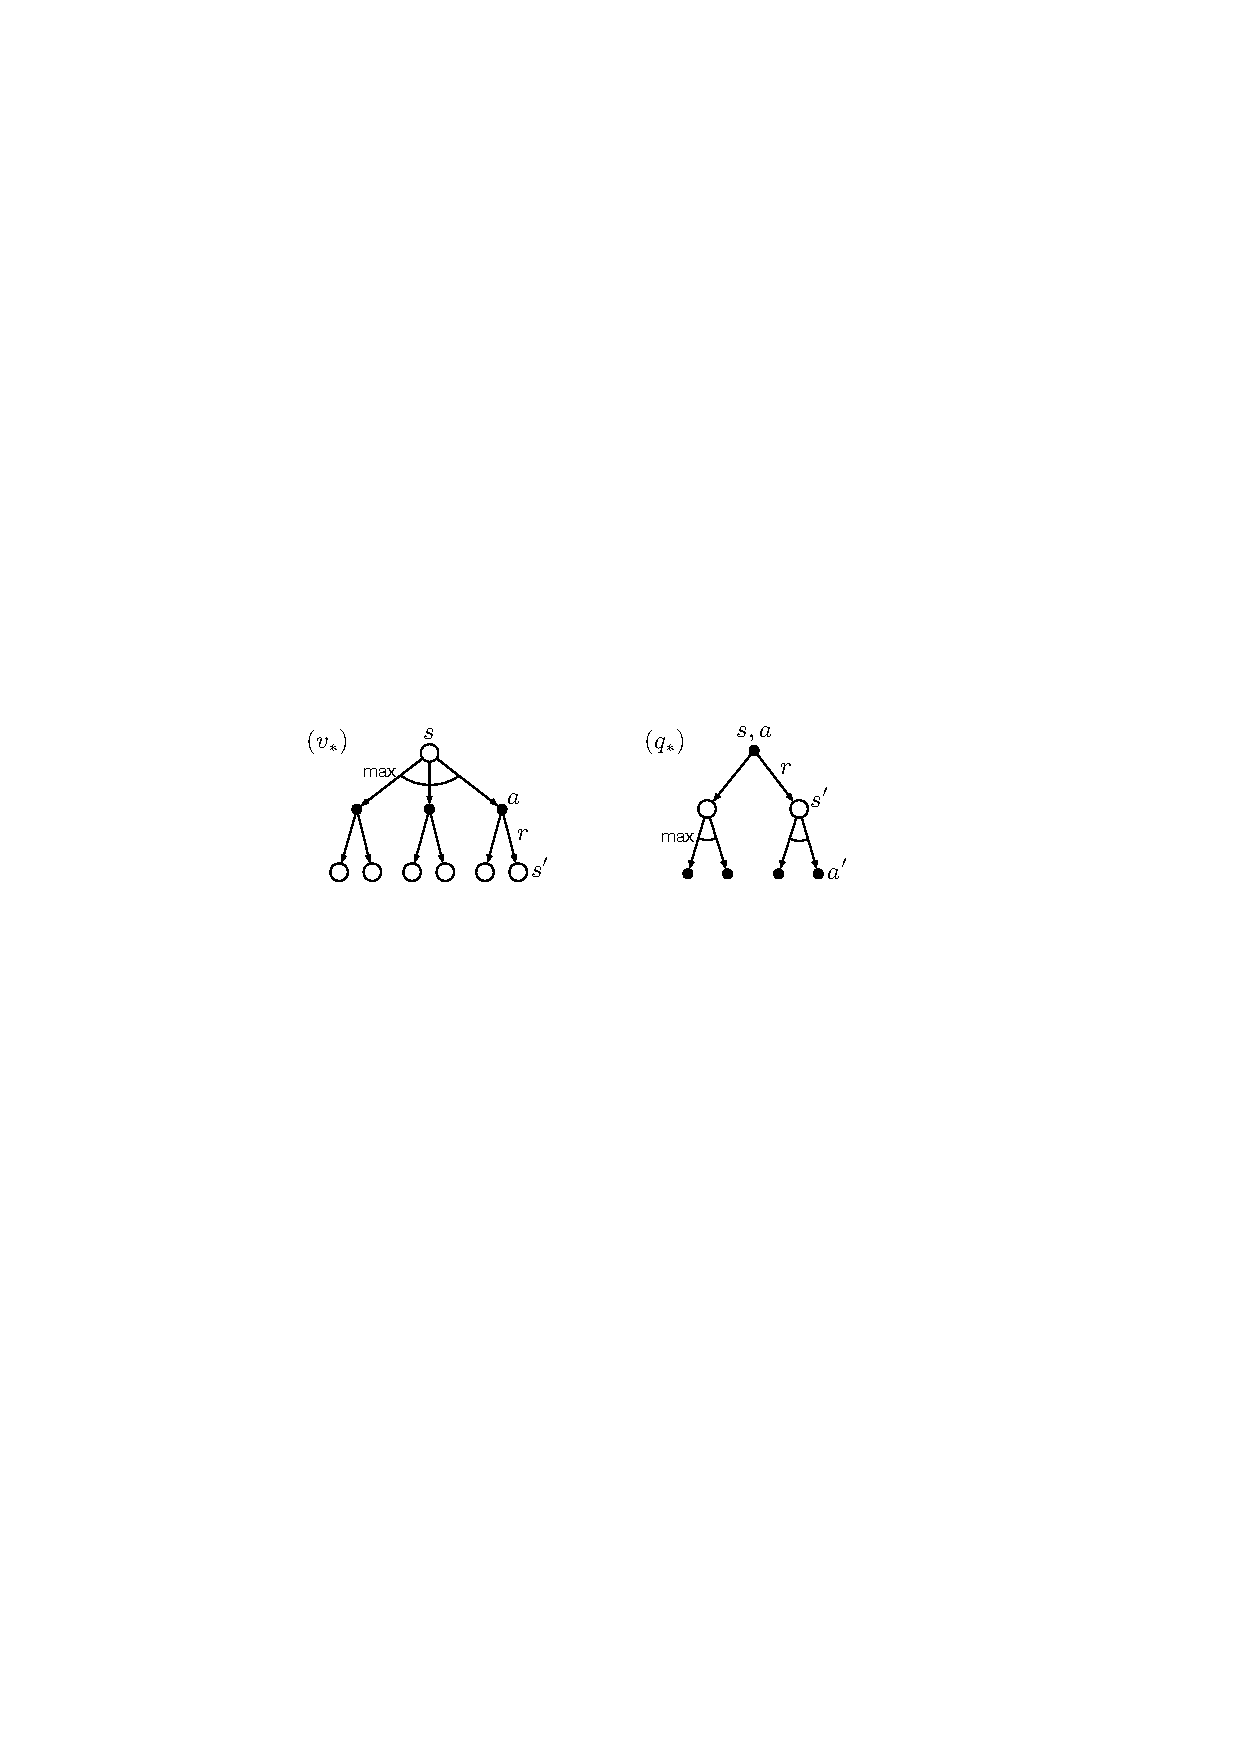
\includegraphics[width=\linewidth{}]{figures/backup.pdf}
  \caption{最適価値関数のバックアップ図 (文献\cite{Sutton1998}より引用) \label{fig:backup}}
\end{figure}

最適状態価値関数$v_{\pi_*}$の下で具体的な
また$v_{\pi_*}$

\begin{align}
  \label{eq:bellman_opt1}
  v_{\pi_*}(s) &= \max_a \sum_{s'}p(s'|s,a)[r(s,a,s') + \gamma v_{\pi_*}(s')] \\
  \label{eq:bellman_opt2}
  q_{\pi_*}(s,a) &= \sum_{s'}p(s'|s,a)[r(s,a,s') +\gamma \max_{a'}q_{\pi_*}(s',a')]
\end{align}

式\ref{eq:bellman_opt1}は最適方策$\pi_*$の下での状態$s$の価値は, すべての行動$a \in A(s)$について$a$を選択した場合の遷移後の状態$s'$の価値と即時報酬の合計を環境のダイナミクスについて期待値を取ったものの最大値であるということを示している.
式\ref{eq:bellman_opt2}も同様に解釈できる.
最適方策の状態価値関数$v_{\pi_*}(s)$, 状態価値関数$q_{\pi_*}(s,a)$をそれぞれ最適状態価値関数, 最適状態行動価値関数という.

\subsection{価値ベースな手法}
価値ベースな手法は価値関数を
Q学習は状態価値関数を以下の更新式~\ref{eq:q_learning}に従って学習するアルゴリズムである.
\begin{align}
  \label{eq:q_learning}
  Q(S_t, A_t) \leftarrow Q(S_t, A_t) + \alpha [R_{t+1} + \gamma \max_a Q(S_{t+1}, a) - Q(S_t, A_t)]
\end{align}


\subsection{方策ベースな手法}

\section{深層強化学習}

\section{AlphaZero}
Silverらが提案したAlphaZero~\cite{AlphaZero}は二人ゼロ和完全確定情報ゲームを対象とした有力な深層強化学習手法である.
囲碁, 将棋, チェスにおいて当時の有力なプログラムを上回る強さを示した.
AlphaZeroは盤面の特徴量を入力として方策と価値を出力するニューラルネットワークを, 自己対戦を通して得たデータから学習する.
自己対戦において, AlphaZeroはモンテカルロ木探索~(MCTS)~というアルゴリズムを使用して指し手を選択する.

MCTSは探索木を構築し, 
MCTSは選択, 展開, 評価, 逆伝播という$4$つのステップを繰り返すことで良い手を選ぶための手法である.
各ノードは

\subsection*{選択}
現在のゲーム木の根ノードから有望な子ノードを選択し, 葉ノードに至るまで辿り続ける.
ここで有望なノードとは暫定の評価の高さと
\subsection*{展開}
\subsection*{評価}
\subsection*{逆伝播}

\section{2048への強化学習の応用}
\subsection{Stochastic MuZero}
